% Name: Row echelon form
% Description: A matrix in row echelon form: each row's leading entry, the pivot, sits to the right of the one above, with only zeros below the staircase.
% Tags: row echelon form, pivots, Gaussian elimination, linear algebra

\usetikzlibrary{matrix}

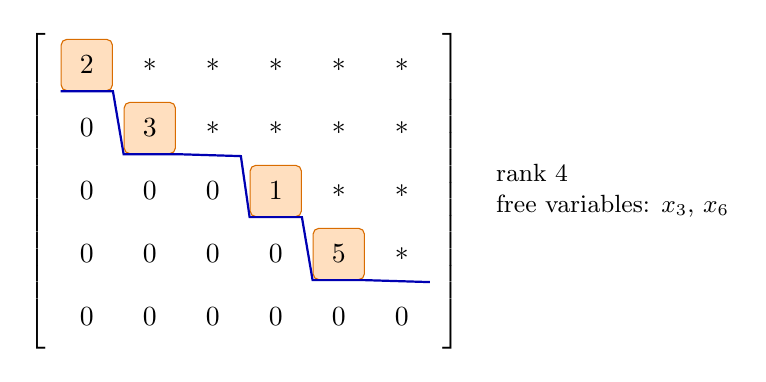
\begin{tikzpicture}[pivot/.style={fill=orange!25, draw=orange!85!black, rounded corners=2pt, inner sep=0pt, minimum size=6.5mm}]
  % Stars are any numbers; pivots in columns 1, 2, 4, and 5
  \matrix (m) [matrix of math nodes, left delimiter={[}, right delimiter={]}, nodes={minimum size=7mm, anchor=center}, column sep=1mm, row sep=1mm] {
    |[pivot]| 2 & * & * & * & * & * \\
    0 & |[pivot]| 3 & * & * & * & * \\
    0 & 0 & 0 & |[pivot]| 1 & * & * \\
    0 & 0 & 0 & 0 & |[pivot]| 5 & * \\
    0 & 0 & 0 & 0 & 0 & 0 \\
  };
  \draw[blue!70!black, thick] (m-1-1.south west) -- (m-1-1.south east) -- (m-2-2.south west) -- (m-2-2.south east) -- (m-2-3.south east) -- (m-3-4.south west) -- (m-3-4.south east) -- (m-4-5.south west) -- (m-4-5.south east) -- (m-4-6.south east);
  \node[right=6mm, font=\small, align=left] at (m.east) {rank $4$ \\ free variables: $x_3$, $x_6$};
\end{tikzpicture}
